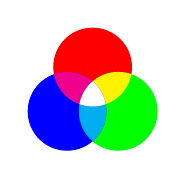
\begin{tikzpicture}
    \def\di{0.5}
    \def\si{0.75*\di}
    \draw [draw=none, fill=red] (90:\si) circle (\di);
    \draw [draw=none, fill=green] (-30:\si) circle (\di);
    \draw [draw=none, fill=blue] (210:\si) circle (\di);
    \begin{scope} % red + green = yellow
        \clip (90:\si) circle(\di);
        \draw [draw=none, fill=yellow] (-30:\si) circle (\di);
    \end{scope} % blue + red = magenta
    \begin{scope}
        \clip (210:\si) circle(\di);
        \draw [draw=none, fill=magenta] (90:\si) circle (\di);
    \end{scope}
    \begin{scope} % green + blue = cyan
        \clip (-30:\si) circle(\di);
        \draw [draw=none, fill=cyan] (210:\si) circle (\di);
    \end{scope}
    \begin{scope} % red + green + blue = white
        \clip (90:\si) circle(\di);
        \clip (210:\si) circle(\di);
        \draw [draw=none, fill=white] (-30:\si) circle (\di);	
    \end{scope}
\end{tikzpicture}